\chapter{System Model}
Cuttlefish, as mentioned earlier, is a 3D printing pipeline, which processes one or more 3D digital models and outputs control code to drive a particular 3D Printer to realize the the object. The digital model of the object to be printed is created either using a modeling software or acquired by 3D scanners. Cuttlefish allows  numerous input file formats like STL, OBJ, PLY, WRL. 

The whole pipeline has a streaming architecture, which means that the input can processed in smaller parts so as to generate the output sooner thus letting the printing process to be started as early as possible i.e. even before the whole object has been processed.The output is generated in parts called as \textit{chunks}- each chunk is a collection of 2D layers, where each layer is referred to as a \textit{slice}. \newline

\section{Non-distributed Cuttlefish Pipeline Components}

The pipeline also has a component-based architecture. The composition of the pipeline varies as per the components assembled to form the pipeline. The components of the pipeline can be chosen on the basis of factors like the type of generated output needed to drive the particular printer, for example \textit{Bitmaproducer} component if the desired output is bitmaps, where as \textit{STLProducerObjet} component is included when the desired output is an STL file per print material, i.e. a mesh representation, or if the output required is a GCode then the component used is \textit{GCodeProducer}, e.g. for FDM printers. Another factor for deciding the components of the pipeline is what attributes of the object should be reproduced: shape, color, translucency, internal structure, etc
\newline

The pipeline performs the following fundamental steps in a serial fashion irrespective of the components forming the pipeline \ref{fig:TypicalCuttlefishSteps}. Let us now examine each of the stages outlined in Figure 3.1:

\begin{figure}[ht!]
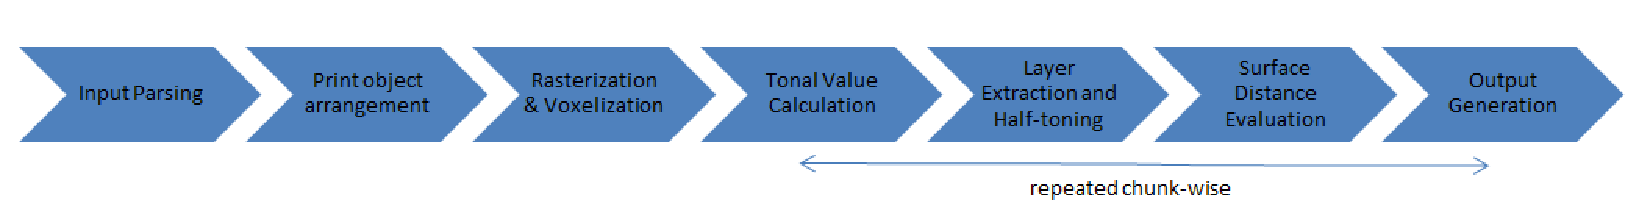
\includegraphics[scale=0.6]{TypicalCuttlefishSteps.pdf}
\caption{Cuttlefish pipeline component functionality}
\label{fig:TypicalCuttlefishSteps}
\end{figure}

\begin{itemize}
\item \textbf{Input Parsing}: The input given to the pipeline, mostly mesh files and textures, is parsed and internal mesh representations are created for them. Internal mesh representations of multiple objects can be grouped into print jobs, together with each having it\textquotesingle s own unique identifier and is referred to as a print object. At present \textit{FileParsePj} is the component which performs this task. \newline 

\item \textbf{Print object arrangement}: The print objects are arranged within the print volume to lower the material consumption and the print time. The arrangement of the print jobs is done by first optimizing the orientation of each print object to reduce print time and support requirements, followed by a greedy approach where in to arrange the print objects (approximated by their bounding boxes) compactly within the print volume. \textit{PrintJobOrganizer} is currently handling this task. \newline 

\item \textbf{Rasterization and Voxelization}: Rasterization is the process of converting vector graphics, e.g. polygons or curves, to raster images,i.e. pixels or dots for output to printer or display device. In our context, the input surface representation is converted to a \textit{voxel} representation-\textit{a voxel is 3D equivalent of 2D pixel}, and each voxel intersecting the surface is assigned attributes like color, occupancy etc. Currently the component doing this is \textit{PrintJobVoxelizer}. The algorithm used for voxelization can be varied using the component configuration and further details are beyond the scope of the thesis. \newline 
 
\item \textbf{Tonal Value Calculation}: This step involves calculation and assignment of tonal values from the optical features (RGB or BRDF data) of surface voxels. The tonal value computation is done with the help of a calculated ICC-profile  belonging to the specific printer. The component doing this is referred to as \textit{TonalValueCalculator}.

\item \textbf{Surface Distance Evaluation and Tonal Analyzer} (optional): The component evaluates the distance of voxels to the surface and assigns values of a given attribute (of the surface voxel)  to inner voxels within the specified maximum distance.The Tonal value analyzer component reports summary statistics, comparing the half-toned signal to the original tonal values in easy to interpret graphs.\newline

\item \textbf{Layer Extraction and Half-toning}: The component \textit{LayerExtractor} extracts the layers below surface which are subsequently half-toned by the component LayerHalftoner. Half-toning is the process of creating an image comprised of discrete dots rather than continuous tones.When viewed from a distance, the dots blur together, creating the illusion of continuous tones. Details can be found in \cite{Brunton}. \newline

\item \textbf{Output Generation}: The generated slices are then used to create the desired output, e.g bitmaps or STL files. The output files are then used to drive the print machine. \newline

\end{itemize} 

The input given to the printer driver is a main configuration file in a \textit{JSON} format - \textit{JSON} (JavaScript Object Notation) is an open-standard format that uses human-readable text to transmit data objects consisting of attribute-value pairs, describing various input fields. The main configuration file lists the files describing the printer specification, component configuration, geometry, appearance, logger type and output folder path. The printer specification file consists of the details related to the resolution of the printer, print volume, material names and unique identifier for each material, \textit{ICC profile}- it is a file which contains data that characterizes any color input/output devices. The component configuration enlists the components forming the pipeline and configuration parameters for each component. Listing \ref{lst:CC} is an example of the \textit{BitmapProducerObjet} component configuration description. \newline

\begin{lstlisting}[label={lst:CC},caption={\textit{BitmapProducerObjet} Component Configuration}]
{
	"type":"BitmapProducerObjet",
  "OutputPath": "Output/",
  "PrinterTextFileName": "printer_config.txt",
  "computeType":"multi-threaded",
  "pitchRequirement": "32",
	"unusedMaterial":"VeroClear"
}
\end{lstlisting}

The \textit{type} field denotes the name of the component and \textit{computeType} sets the component to run in a single-threaded or multi-threaded fashion. \textit{OutputPath} is used to set the path at which the component generates the bitmaps and \textit{pitchRequirement} value is used to make the bitmap width a multiple of the specified number. The component which parses the input main configuration file creates a \textit{PrintingSoftware} for the given component configuration. 

\section{System Model for Distributed Cuttlefish Pipeline} \label{sysMod}

The non-distributed cuttlefish pipeline runs on a single machine and therefore there is no particular machine specific action needed to be performed depending on the role of the machine. For an application to run on a cluster of machines, sometimes it is necessary to perform additional steps which are specific to the role of the node in the cluster. Before understanding the architecture of the distributed cuttlefish printer driver it is necessary to understand the architecture of the cluster, referred to as a distributed system, on which the driver is designed to run. 

\subsection{Distributed system for cuttlefish printer driver} \label{clusterArch}

The distributed cuttlefish printer driver is developed using a cluster of the computers(nodes) which are heterogeneous in their hardware as well as software configuration and are connected via a standard workplace network. The initial set up used during the development had three nodes out of which one node is the master node and remaining nodes are the slave nodes. The names master and slave depict a predetermined role the nodes have and type of work they do. The nodes also have access to a shared networked file system (figure \ref{fig:CuttlefishCluster}).

\begin{figure}[ht!]
\centering
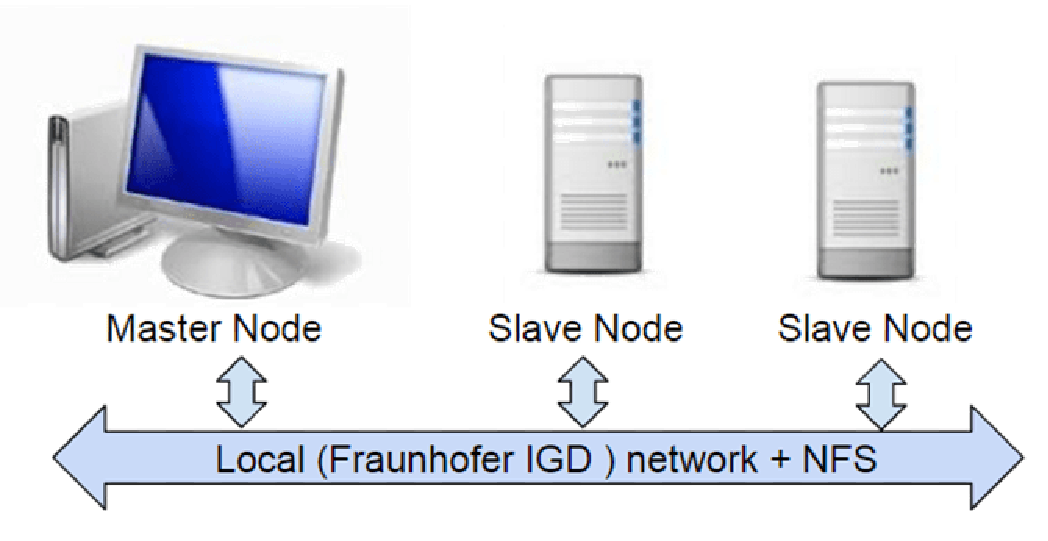
\includegraphics[scale=0.6]{CuttlefishCluster.pdf}
\caption{Cluster setup}
\label{fig:CuttlefishCluster}
\end{figure}

As mentioned earlier, the role of the node determines the type of work they do.The master node is the computer in the cluster where the user submits his request, namely the main configuration file (figure \ref{fig:Step1}). 

\begin{figure}[ht!]
\centering
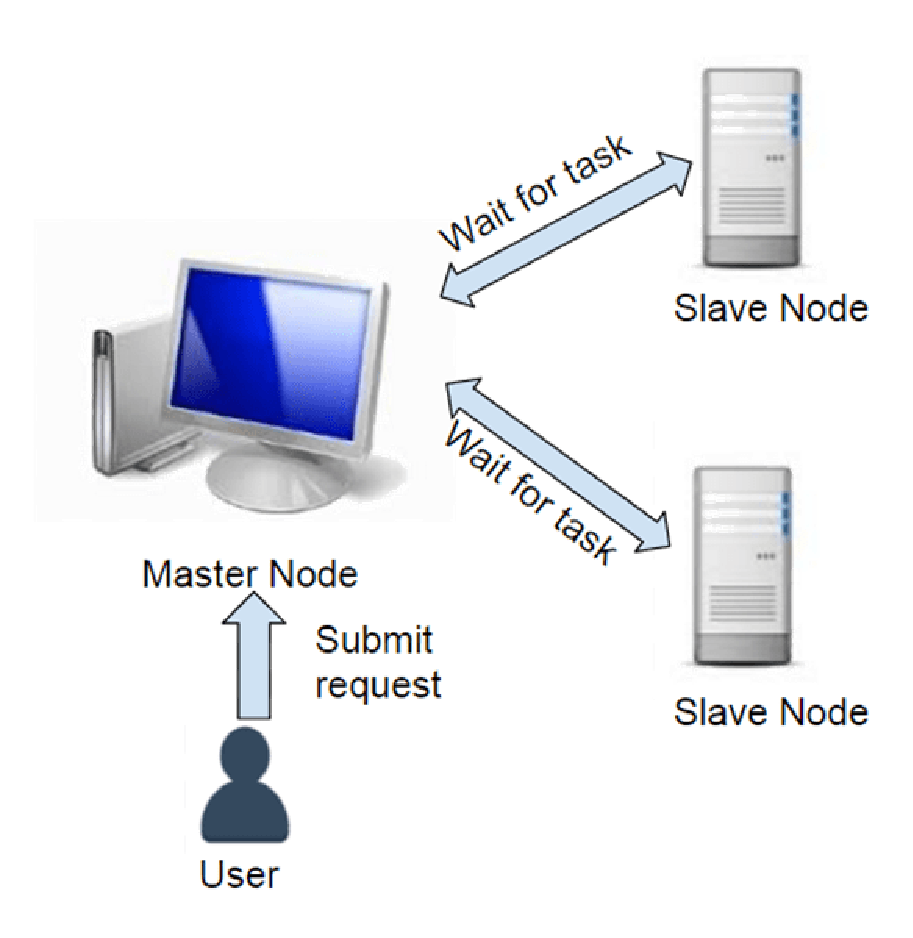
\includegraphics[scale=0.6]{Step1.pdf}
\caption{User submits the request}
\label{fig:Step1}
\end{figure}

The master node then performs some computation and distributes the sub-tasks to be performed by the slave nodes (figure \ref{fig:Step2}). 

\begin{figure}[ht!]
\centering
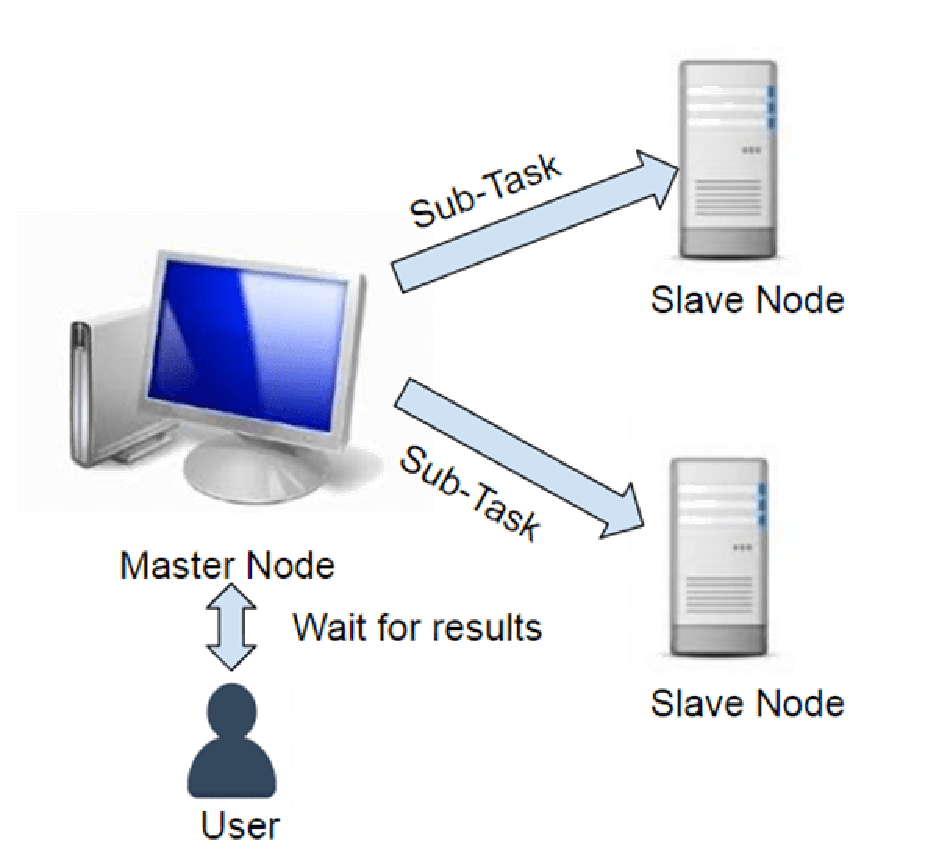
\includegraphics[scale=0.6]{Step2.pdf}
\caption{Master distributes the sub-tasks}
\label{fig:Step2}
\end{figure}

The slave nodes perform the assigned tasks and report back to the master (figure \ref{fig:Step3}). The cluster nodes follow a classic \textit{master-slave} communication paradigm. 

\begin{figure}[ht!]
\centering
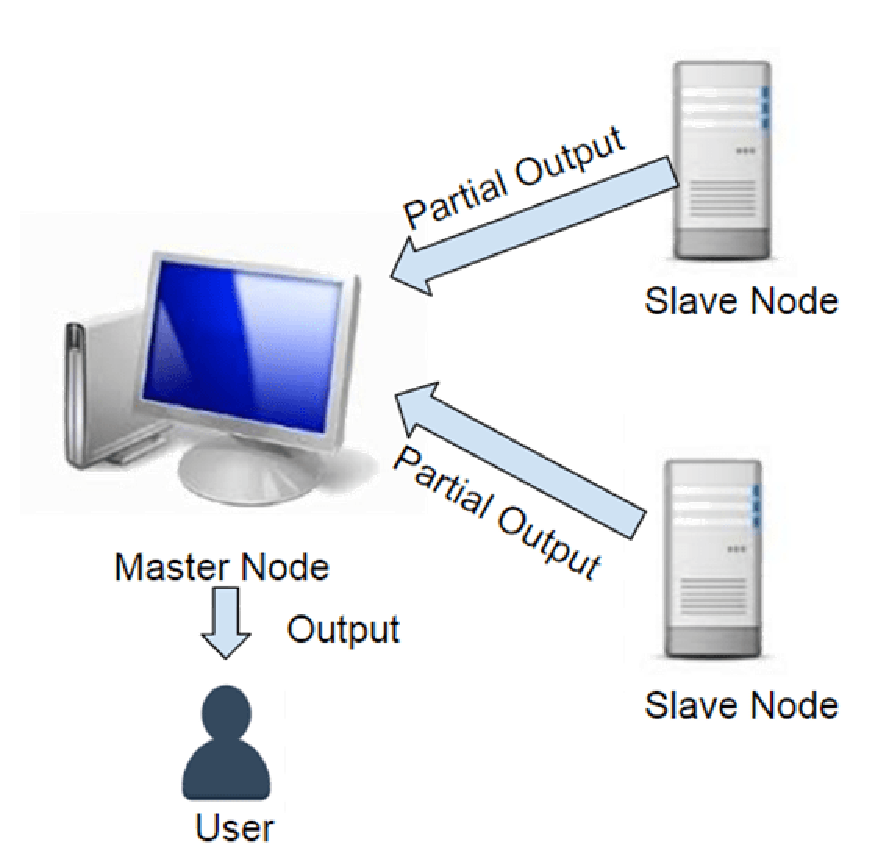
\includegraphics[scale=0.6]{Step3.pdf}
\caption{Slaves report the partial output}
\label{fig:Step3}
\end{figure}

\subsection{Components of distributed cuttlefish printer driver} \label{DSCuttlefish}

The distributed cuttlefish pipeline components may differ depending upon the role of the node in the cluster. The components put together form a printing software in which the components run on the node in a loop, with each iteration of the loop processing chunk-wise data. To apply distributed computing as a solution for stated problem of large computation on big data set, there are three additional steps, as enlisted below, some of which need to be performed either on the master or the slave node:  
\begin{enumerate}
\item Division of task into sub-tasks 
\item Awaiting the sub-tasks and doing the needed work
\item Submitting back the partial output
\end{enumerate}

\subsubsection{Master Node Printing Software Components}

\begin{figure}[t]
\centering
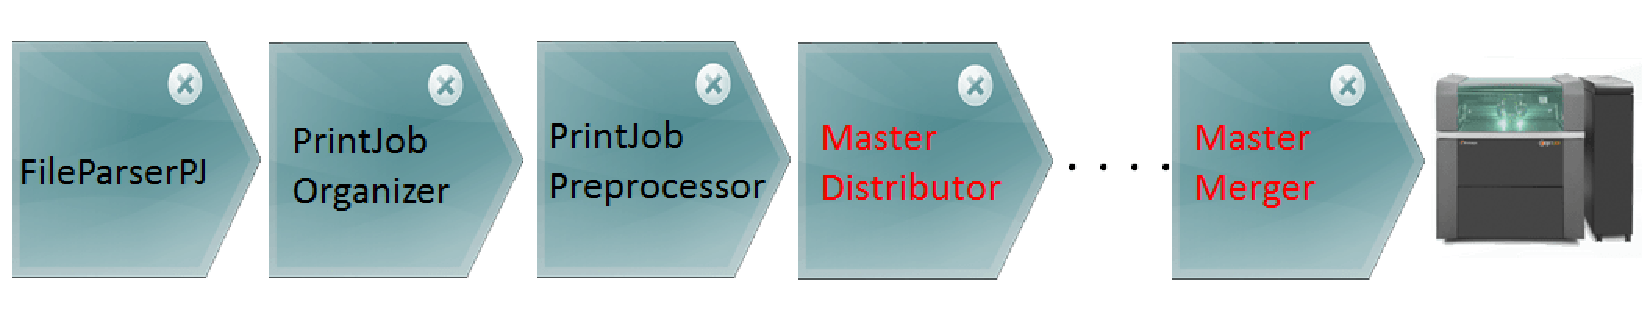
\includegraphics[scale=0.6]{MasterPSPl.pdf}
\caption{Master Node Printing Software Components For Prototype I}
\label{fig:MasterPS}
\end{figure}

As per the model discussed in the section \ref{clusterArch}, the master node performs the step $1$ from the above steps. The division of the task among the slave nodes needs to be performed by the master efficiently so as to make sure that distributed load is balanced and none of the slaves are over-worked. To do so, the master needs to evaluate the input and perform some measurements so as to make a wise decision regarding the task split. Hence, the master printing software needs to at least parse the input into an internal mesh representation i.e. print jobs and compute the necessary parameters on the basis of which an informed decision can be made. The component \textit{MasterDistributor} is responsible for division of the submitted task and takes the print jobs as input and generates sub-tasks as the output. After the successful generation of the sub-tasks, the distribution of the sub-tasks among the slaves is done. The form in which the tasks are distributed may vary leading to different designs of the component which is discussed in detail in the next chapter. 

\begin{figure}[t]
\centering
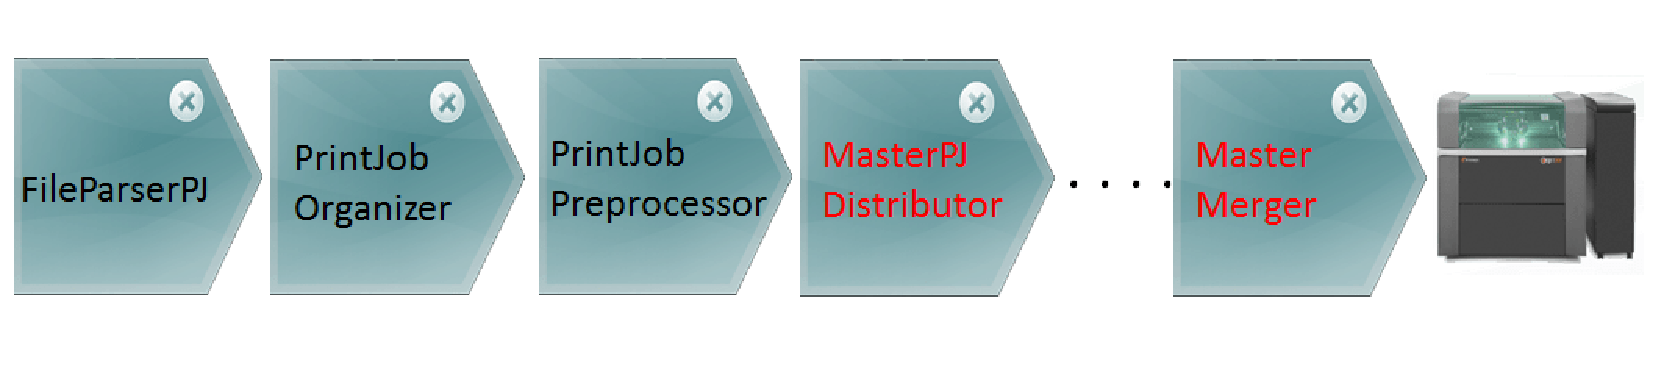
\includegraphics[scale=0.6]{MasterPSPIl.pdf}
\caption{Master Node Printing Software Components For Prototype II}
\label{fig:MasterPSII}
\end{figure}

On receiving the sub-tasks from the master, the slave nodes start doing their share of work. The master after submitting the sub-tasks has to wait for the slaves to generate the partial output. So as to maintain the streaming architecture, the slaves perform the assigned work in chunks and report the partial output to the master. The master then collects the partial output and performs some computation using received data and provides the final output to the user. \textit{MasterMerger} component in the master printing pipeline is responsible for receiving the partial output from all the slaves and combining it before sending it on to the output component. The output from the slave nodes are the chunks of partial \textit{slices} which are later merged into chunks of full slices. Figure \ref{fig:MasterPS} shows the components of the printing software running on the master node for Prototype I and Figure \ref{fig:MasterPSII} for prototype II .

\subsubsection{Slave Node Printing Software Components }

\begin{figure}[b]
\centering
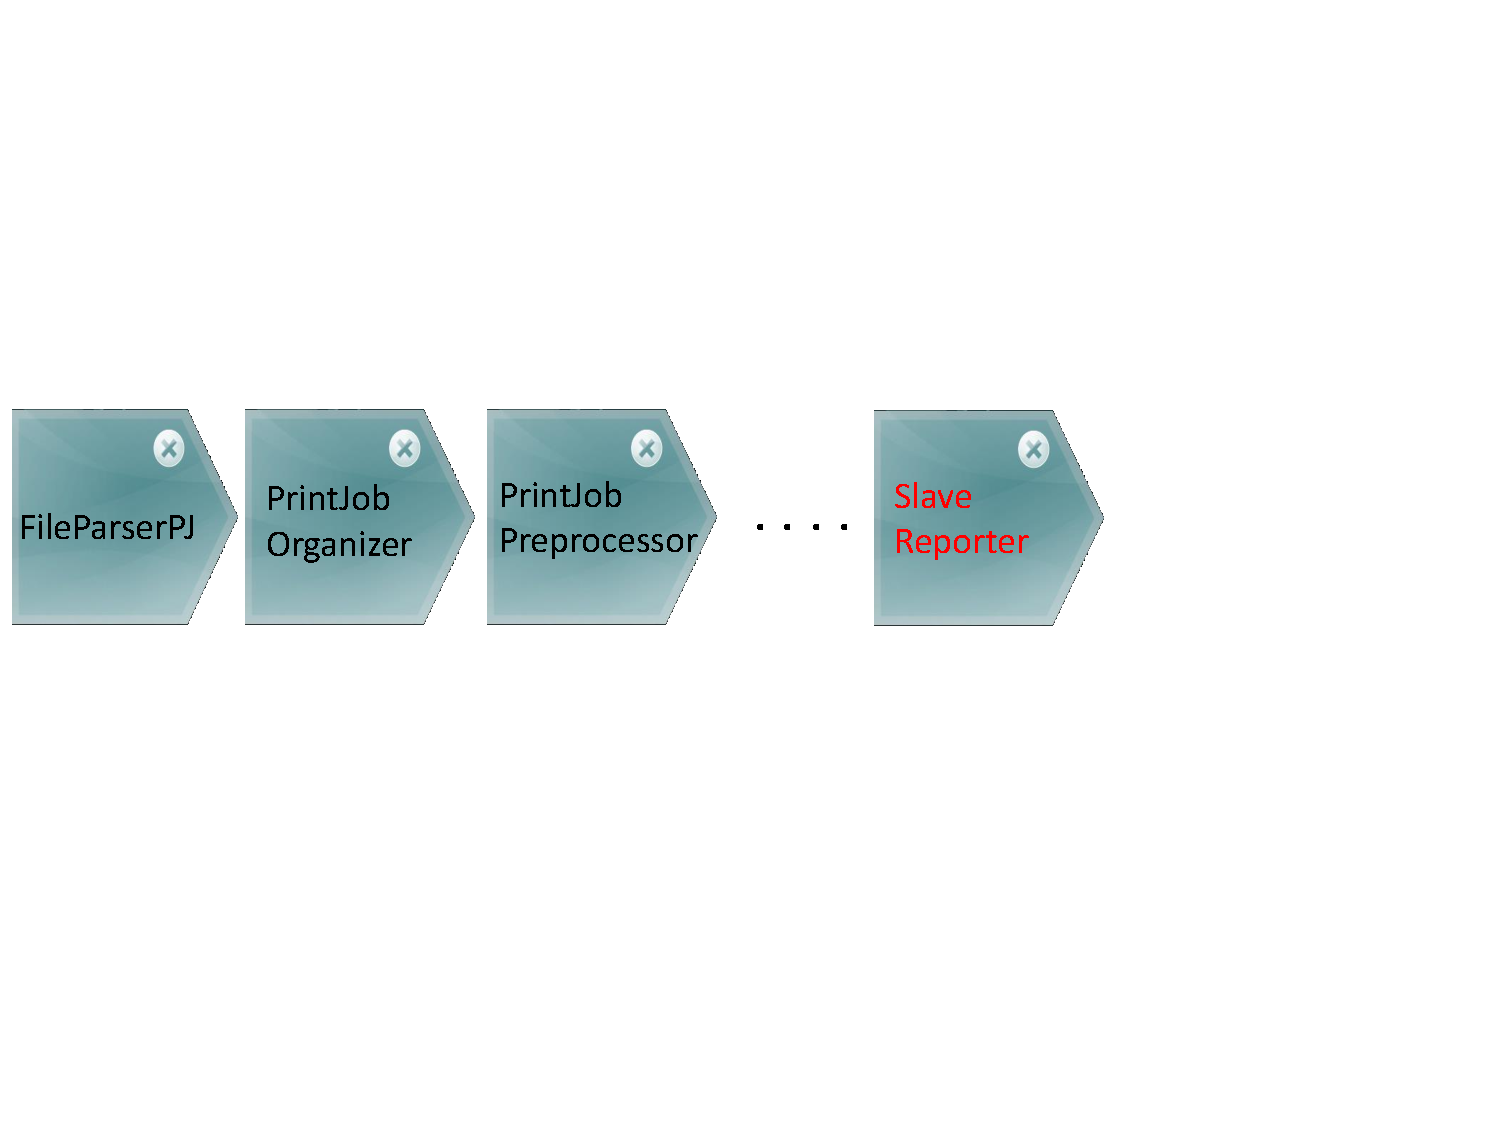
\includegraphics[scale=0.6]{SlavePSPI.pdf}
\caption{Slave Node Printing Software Components For Prototype I }
\label{fig:SlavePS}
\end{figure}

The slave nodes in the cluster (i.e. all nodes other than the master are considered slave nodes) perform the assigned task and report back the results to the master node. To do so, the slaves nodes have to first wait until the master has divided the task submitted by the user into smaller sub-tasks. Once receiving the input, the slave nodes run the whole printing software (similar to the non-distributed cuttlefish version) with just one minor change. As the slave nodes report the partial output to the master, they do not need to run the output component, for example the \textit{Bitmapproducer}. The partial output which is reported by the slaves to master is in form of \textit{slices} and hence, the slave printing software running on the slave nodes does not contain the output component, instead it runs a component called the \textit{SlaveReporter} which, as the name suggests, reports the partial output in a chunk-wise fashion back to the master. Figure \ref{fig:SlavePS} shows the components of the printing software running on the slave node for Prototype I and Figure \ref{fig:SlavePSII} for Prototype II.

\begin{figure}[t]
\centering
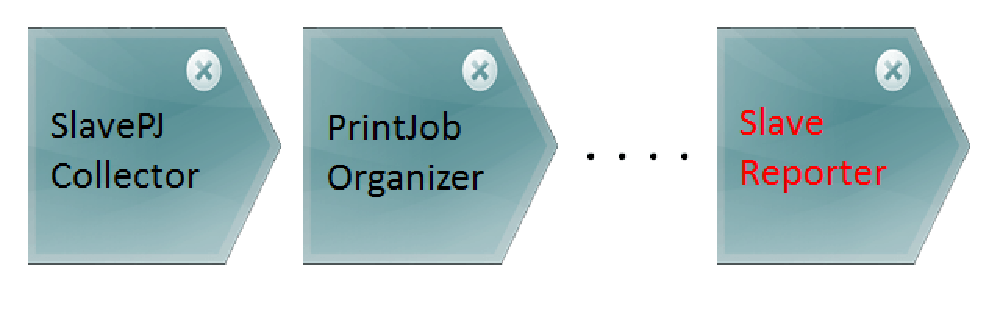
\includegraphics[scale=0.6]{SlavePSPII.pdf}
\caption{Slave Node Printing Software Components For Prototype II }
\label{fig:SlavePSII}
\end{figure}

\clearpage
